\documentclass{scinote}

%%%%%%%%%%%%%%%%%%% tikz %%%%%%%%%%%%%%%%%

\usepackage{standalone}
\usepackage{tkz-graph}
\usetikzlibrary{calc}
\usetikzlibrary{positioning}
% add figure path for graphicx
\graphicspath{{figure/}}

% quote \enquote{}
\usepackage[autostyle]{csquotes}


%%%%%%%%%%%%%%%%%%% math %%%%%%%%%%%%%%%%%
\usepackage{fixmath}
\usepackage{mathtools}
%%%%%%%%%%%%%%%%%%% biblatex %%%%%%%%%%%%%%%%%

%%%%%%%%%%%%%%%%%%%%% glossaries %%%%%%%%%%%%%%%%%
\setlength{\glsdescwidth}{1\linewidth}

\renewcommand\glossaryname{List of Abbreviations and Symbols}

\newglossaryentry{Q2}{name={$Q_2\left(f\right)$},
	%sort=Q2,
	description={Two-side (bounded) error quantum query complexity}}

\newglossaryentry{real_number}{name={$\mathbb{R}$},description={Real number}}

\newglossaryentry{v}{name={$\vec{v}$},description={a vector}}

% physics
\newglossaryentry{hamiltonian}{name={$\hat{H}$},description={Hamiltonian}}
\newglossaryentry{lagrangian}{name={$L$},description={Lagrangian}}

\newacronym{gcd}{GCD}{Greatest Common Divisor}

\newacronym{qft}{QFT}{Quantum Field Theory}
\newacronym{qm}{QM}{Quantum Mechanics}

% machine learning
\newacronym{gd}{GD}{Gradient Descent}
\newacronym{svm}{SVM}{Support Vector Machine}
\newacronym{mle}{MLE}{Maximum Likelihood Estimation}
\newacronym{map}{MAP}{Maximum A Posteriori Estimation}
\newacronym{pdf}{PDF}{Probability Density Function}
\newacronym{em}{EM}{Expectation Maximum}
\newacronym{gmm}{GMM}{Gaussian Mixture Model}
\newacronym{kl}{KL}{Kullback-Leibler}
\newacronym{vae}{VAE}{Variational Autoencoder}

% gan
\newacronym{gan}{GAN}{Generative Adversarial Nets}
\newacronym{cgan}{CGAN}{Conditional Generative Adversarial Nets}
\newacronym{dcgan}{DCGAN}{deep convolutional GAN}
\newacronym{wgangp}{WGAN-GP}{Wasserstein GAN with Gradient Penalty}

% autoregressvie model
\newacronym{rnn}{RNN}{Recurrent Neural Network}
\newacronym{lstm}{LSTM}{Long Short-Term Memory}
\newacronym{gru}{GRU}{Gated Recurrent Unit}

% diffusion models
\newacronym{ddm}{DDM}{Denoising Diffusion Models}
\newacronym{ddim}{DDIM}{Denoising Diffusion Implicit Models}

\newacronym{bert}{BERT}{Bidirectional Encoder Representations from Transformers}

\makeglossaries
%%%%%%%%%%%%%%%%%%%%% glossaries %%%%%%%%%%%%%%%%%

\usepackage{xargs}
\usepackage[colorinlistoftodos,prependcaption,textsize=tiny]{todonotes}
\newcommandx{\unsure}[2][1=]{\todo[linecolor=red,backgroundcolor=red!25,bordercolor=red,#1]{#2}}
\newcommandx{\change}[2][1=]{\todo[linecolor=blue,backgroundcolor=blue!25,bordercolor=blue,#1]{#2}}
\newcommandx{\info}[2][1=]{\todo[linecolor=purple,backgroundcolor=purple!25,bordercolor=purple,#1]{#2}}
\newcommandx{\improvement}[2][1=]{\todo[linecolor=green,backgroundcolor=green!25,bordercolor=green,#1]{#2}}
\newcommandx{\thiswillnotshow}[2][1=]{\todo[disable,#1]{#2}}

% math
\let\iff\relax
\newcommand{\iff}{\text{ iff }}
\newcommand{\OPT}{\textup{OPT}}

\DeclareRobustCommand\transp{^{\mathrm{T}}}

% lowercase italic for variables: x ($x$)
% lowercase italic bold for vectors: x ($\mathbold{x}$)
% uppercase italic bold for matrices: X ($\mathbold{X}$)
% uppercase italic for random variables: X ($X$)

\renewcommand{\vec}[1]{\ensuremath{\mathbold{#1}}}
\newcommand{\mat}[1]{\ensuremath{\mathbold{#1}}}
\newcommand{\vx}{\ensuremath{\vec{x}}}
\newcommand{\vX}{\ensuremath{\mat{X}}}

\DeclareMathOperator*{\argmax}{arg\!\max}
\DeclareMathOperator*{\argmin}{arg\!\min}

\makeatletter
\newcommand{\@giventhatstar}[2]{\left(#1\;\middle|\;#2\right)}
\newcommand{\@giventhatnostar}[3][]{#1(#2\;#1|\;#3#1)}
\newcommand{\giventhat}{\@ifstar\@giventhatstar\@giventhatnostar}
\makeatother

\newcommand{\pautoref}[1]{(\autoref{#1})}


%%%%%%%%%%%%%%%%%%%%%%%%%%%%%%%%%%%%%%%%%%%%%%%%%%
%%%%%%%%%%%%%%%% begin of document %%%%%%%%%%%%%%%
%%%%%%%%%%%%%%%%%%%%%%%%%%%%%%%%%%%%%%%%%%%%%%%%%%

\makeatletter
\newcommand{\email}[1]{%
	\def\@email{#1}%
}
\makeatother


\begin{document}

\title{\bf \huge Study Notes}
\author{Yangyang Li \\ \href{mailto:yangyang.li@northwestern.edu}{yangyang.li@northwestern.edu}}

\date{Update on \today}
\maketitle
\setcounter{tocdepth}{2}
\setcounter{minitocdepth}{1}
\setlist[enumerate]{itemsep=0mm}
\setlist[itemize]{itemsep=0mm}

\begin{multicols}{2}
	\dominitoc% Initialization
	\adjustmtc[2]% chp number shift for mini-toc
	\tableofcontents
	\label{toc-contents}
\end{multicols}

\listoffigures
% \listoftables
\begin{multicols}{2}
	\listoftheorems[ignoreall,show={theorem}]
\end{multicols}

\renewcommand{\listtheoremname}{List of Definitions}
\begin{multicols}{2}
	\listoftheorems[ignoreall,show={definition}]
\end{multicols}

\printglossaries
% \printglossary[type=\acronymtype]
% \printglossary
% \printglossary[title=List of terms, toctitle=List of terms]

%https://github.com/cauliyang/Latex-Template-for-Scientific-Style-Book.git bib2gls
% \printunsrtglossaries % print all types
% \printunsrtglossary[type={abbreviations},title=List of Abbreviations,style=listgroup]
% \printunsrtglossary[type={abbreviations},title=List of Abbreviations,style=listhypergroup] % doesn't work
% \printunsrtglossary[type={symbols},title=List of Symbols,style=listgroup]
% \printunsrtglossary % main entry

%%%%%%%%%%%%%%%Content%%%%%%%%%%%%%%%
% \mainmatter % separat the number of toc and mainmatter
\chapter*{Preface}
\addcontentsline{toc}{chapter}{Preface}

\minitoc

% % \lipsum % dummy text - remove from real document

\section{Features of this template}
% \epigraph{\emph{... nature isn't classical, dammit, and if you want to make a simulation of nature, you'd better make it quantum mechanical, and by golly it's a wonderful problem, because it doesn't look so easy.}}{Richard Feynman (1981) Simulating physics with computers}
\epigraph{\emph{TeX, stylized within the system as \LaTeX, is a typesetting system which was designed and written by Donald Knuth and first released in 1978. TeX is a popular means of typesetting complex mathematical formulae; it has been noted as one of the most sophisticated digital typographical systems.}}{- \href{https://en.wikipedia.org/wiki/TeX}{Wikipedia}}

\subsection{crossref}
different styles of clickable definitions and theorems
\begin{itemize}
	\item nameref:
	      \nameref{def:gaussian_distribution}

	\item autoref:
	      \autoref{def:gaussian_distribution},
	      \autoref{alg:miller_rabin}

	\item cref:
	      \cref{def:gaussian_distribution},

	\item hyperref:
	      \hyperref[def:gaussian_distribution]{Gaussian},
\end{itemize}

\subsection{ToC (Table of Content)}
\begin{itemize}
	\item mini toc of sections at the beginning of each chapter
	\item list of theorems, definitions, figures
	\item the chapter titles are bi-directional linked
\end{itemize}

\subsection{header and footer}
fancyhdr
\begin{itemize}
	\item right header: section name and link to the beginning of the section
	\item left header: chapter title and link to the beginning of the chapter
	\item footer: page number linked to ToC of the whole document
\end{itemize}

\subsection{bib}
\begin{itemize}
	\item titles of reference is linked to the publisher webpage e.g., \cite{kitaev2002classical}
	\item backref (go to the page where the reference is cited) e.g., \cite{childsUniversalComputationQuantum2009}
	\item customized video entry in reference like in \cite{babaiGraphIsomorphismQuasipolynomial2016}
\end{itemize}

\subsection{preface, index, quote (epigraph) and appendix}
\myindex{index} page at the end of this document...

% \subsection{symbol and glossary (abbreviation)}
% examples:
% \gls{real_number},
% % \gls{natural_number},
% % \gls{complex_number},
% \gls{svm},
% \gls{v}

% \subsubsection{usage}
% \begin{itemize}
% 	\item glossary package
% 	      \begin{verbatim}
% 		pdflatex scinote.tex
% 		makeglossaries scinote
% 		pdflatex scinote.tex
% 	\end{verbatim}

% 	\item glossary-extra package and bib2gls
% 	      \begin{verbatim}
% 		pdflatex scinote.tex
% 		bib2gls scinote
% 		pdflatex scinote.tex
% 	\end{verbatim}
% \end{itemize}

% \section{Related Tools}
% \subsection{VSCode}
% Extension: \href{https://marketplace.visualstudio.com/items?itemName=James-Yu.latex-workshop}{Latex Workshop by James Yu}

% \subsubsection{settings}

% \subsection{lualatex and latexmk}
% .latexmkrc configuration file
% \begin{verbatim*}
% 	$pdflatex = 'lualatex -synctex=1 -interaction=nonstopmode --shell-escape %O %S';
% 		@generated_exts = (@generated_exts, 'synctex.gz');
% 	$pdf_mode = 1;

% 	add_cus_dep('glo', 'gls', 0, 'makeglo2gls');
% 	sub makeglo2gls {
% 			system("makeindex -s '$_[0]'.ist -t '$_[0]'.glg -o '$_[0]'.gls '$_[0]'.glo");
% 		}
% \end{verbatim*}
% To explain ....
% \begin{verbatim}
% # Also delete the *.glstex files from package glossaries-extra. Problem is,
% # that that package generates files of the form "basename-digit.glstex" if
% # multiple glossaries are present. Latexmk looks for "basename.glstex" and so
% # does not find those. For that purpose, use wildcard.
% $clean_ext = "%R-*.glstex";

% push @generated_exts, 'glstex', 'glg';

% add_cus_dep('aux', 'glstex', 0, 'run_bib2gls');

% # PERL subroutine. $_[0] is the argument (filename in this case).
% # File from author from here: https://tex.stackexchange.com/a/401979/120853
% sub run_bib2gls {
%     if ( $silent ) {
%     #    my $ret = system "bib2gls --silent --group '$_[0]'"; # Original version
%         my $ret = system "bib2gls --silent --group $_[0]"; # Runs in PowerShell
%     } else {
%     #    my $ret = system "bib2gls --group '$_[0]'"; # Original version
%         my $ret = system "bib2gls --group $_[0]"; # Runs in PowerShell
%     };

%     my ($base, $path) = fileparse( $_[0] );
%     if ($path && -e "$base.glstex") {
%         rename "$base.glstex", "$path$base.glstex";
%     }

%     # Analyze log file.
%     local *LOG;
%     $LOG = "$_[0].glg";
%     if (!$ret && -e $LOG) {
%         open LOG, "<$LOG";
%     while (<LOG>) {
%             if (/^Reading (.*\.bib)\s$/) {
%         rdb_ensure_file( $rule, $1 );
%         }
%     }
%     close LOG;
%     }
%     return $ret;
% }
% \end{verbatim}

% \subsection{Zotero and Better-bibtex}
% [todo]
% https://retorque.re/zotero-better-bibtex/
% customized entry, e.g., \textbf{Online Video}

% \section{Copyright and License}

% \begin{itemize}
% 	\item GitHub Repo: \url{https://github.com/cauliyang/Latex-Template-for-Scientific-Style-Book}
% 	\item Overleaf template: \url{https://www.overleaf.com/latex/templates/latex-template-for-scientific-style-book/ntprxjksmqxx}
% \end{itemize}


\part{Machine Learning}
\chapter{Probability}\label{chp:Probability}
\minitoc

\section{Basic Concepts}

% https://stanford.edu/~shervine/teaching/cs-229/refresher-probabilities-statistics

Permutation is an arrangement of objects in which the order is important.

\[
	P\left(n,r\right)=  \frac{n!}{\left(n-r\right)!}
\]

Combination is an arrangement of objects in which the order is not important.


\[
	C\left(n,r\right) = \frac{P\left(n,r\right)}{r!} = \frac{n!}{r!\left(n-r\right)!}
\]

in which \(0 \le r \le n\).


% https://github.com/cauliyang/Machine-Learning-Session/blob/master/
\section{Maximum Likelihood Estimation}

\begin{equation}
	\vX = (\vx_1, \vx_2, \dots, \vx_N)\transp, \vx_i = (x_{i1}, x_{i2},\dots, x_{ip})\transp
\end{equation}
in which $N$ is the number of samples, $p$ is the number of features.
The data is sampled from a distribution $p\giventhat{\vx}{\theta}$, where $\theta$ is the parameter of the distribution.


For \(N\)  i.i.d. samples, the likelihood function is \(p \giventhat{\vX}{\theta} = \prod_{i=1}^{N} p \giventhat{\vx_i}{\theta}) \)

In order to get \(\theta\), we use \gls{mle}  to maximize the likelihood function.

\begin{equation}
	\theta_{\mathtt{MLE}} = \argmax_{\theta} \log p\giventhat{\vX}{\theta} = \argmax_{\theta} \sum_{i=1}^{N} \log p\giventhat{\vx_i}{\theta}
\end{equation}

\section{Maximum A Posteriori Estimation}
In Bayes' theorem, the \(\theta\) is not a constant value, but \(\theta \sim  p(\theta) \).
Hence,

\begin{equation}
	p\giventhat{\theta}{\vX} = \frac{p\giventhat{\vX}{\theta} p(\theta)}{p(\vX)}  =  \frac{p\giventhat{\vX}{\theta} p(\theta)}{\int\limits_{\theta} p\giventhat{\vX}{\theta} p(\theta) d\theta}
\end{equation}


In order to get \(\theta\), we use \gls{map}  to maximize the posterior function.

\begin{equation}
	\theta_{\mathtt{MAP}} = \argmax_{\theta} p\giventhat{\theta}{\vX} = \argmax_{\theta} \frac{p\giventhat{\vX}{\theta} p(\theta)}{p(\vX)}
\end{equation}


After \(\theta\) is estimated, then  calculating \(\frac{p\giventhat{\vX}{\theta} \cdot p(\theta)}{\int\limits_{\theta} p\giventhat{\vX}{\theta} p(\theta) d\theta}\) to get the posterior distribution.
We can use the posterior distribution to predict the probability of a new sample \(\vx\).


\begin{equation}
	p \giventhat{x_{\mathtt{new}}}{\vX}  = \int\limits_{\theta} p\giventhat{x_{\mathtt{new}}}{\theta} \cdot p\giventhat{\theta}{\vX} d\theta
\end{equation}

\section{Gaussian Distribution}

Gaussian distribution is also called normal distribution.

\begin{equation}
	\boldsymbol{\theta} = (\mu, \sigma^2), \quad \mu = \frac{1}{N} \sum_{i=1}^{N} x_i, \quad \sigma^2 = \frac{1}{N} \sum_{i=1}^{N} (x_i - \mu)^2
\end{equation}

For \gls{mle},

\begin{equation}
	\boldsymbol{\theta} = (\mu, \Sigma) = (\mu, \sigma^2), \quad \theta_{\mathtt{MLE}} = \argmax_{\theta} \log p\giventhat{\vX}{\theta} = \argmax_{\theta} \sum_{i=1}^{N} \log p\giventhat{\vx_i}{\theta}
\end{equation}


Generally, the \gls{pdf} of a Gaussian distribution is:

\begin{equation}
	p\giventhat{x}{\mu, \Sigma} =  \frac{1}{\sqrt{(2\pi)^p \det(\Sigma)}} \exp\left(-\frac{1}{2} (\vx - \mu)\transp \Sigma^{-1} (\vx - \mu)\right)
\end{equation}
in which \(\mu\) is the mean vector, \(\Sigma\) is the covariance matrix, \(\det\) is the determinant of matrix.
\(\det\)  is the product of all eigenvalues of a matrix.

Hence,

\begin{equation}
	\log p\giventhat{\vX}{\theta}  = \sum_{i=1}^{N} \log p\giventhat{x_i}{\theta} = \sum_{i=1}^{N} \log \frac{1}{\sqrt{(2\pi)^p \det(\Sigma)}} \exp\left(-\frac{1}{2} (\vx - \mu)\transp \Sigma^{-1} (\vx - \mu)\right)
\end{equation}

Let's only consider 1 dimension case for brevity, then

\begin{equation}
	\log p\giventhat{\vX}{\theta}  = \sum_{i=1}^{N} \log p\giventhat{x_i}{\theta} = \sum_{i=1}^{N} \log \frac{1}{\sqrt{2\pi \sigma^2}} \exp\left(-\frac{1}{2} \frac{(x - \mu)^2}{\sigma^2}\right)
\end{equation}

Let's get the optimal value for \(\mu\),

\begin{equation}
	\mu_{\mathtt{MLE}} = \argmax_{\mu} \log p\giventhat{\vX}{\theta} = \argmin_{\mu} \sum_{i=1}^{N} \frac{1}{2} \left(x_i - \mu\right)^2
\end{equation}

So,

\begin{equation}
	\frac{\partial \log p\giventhat{\vX}{\theta}}{\partial \mu} = \sum_{i=1}^{N} \left(\mu - x_i\right) = 0 \rightarrow \mu_{\mathtt{MLE}} = \frac{1}{N} \sum_{i=1}^{N} x_i
\end{equation}


Let's get the optimal value for \(\sigma^2\),

\begin{align*}
	\sigma_{\mathtt{MLE}} & = \argmax_{\sigma} \log p\giventhat{\vX}{\theta}                                                                                \\
	                      & =\argmax_{\sigma} \sum_{i=1}^{N} \log \frac{1}{\sqrt{2\pi \sigma^2}} \exp\left(-\frac{1}{2} \frac{(x - \mu)^2}{\sigma^2}\right) \\
	                      & = \argmax_{\sigma} \sum_{i=1}^{N} \left[ - \log\sqrt{2\pi \sigma^2} - \frac{(x - \mu)^2}{2\sigma^2} \right]                     \\
	                      & = \argmin_{\sigma} \sum_{i=1}^N \left[ \log \sigma + \frac{\left(x - \mu\right)^2}{2\sigma^2}\right]                            \\
\end{align*}

Hence,

\begin{equation}
	\frac{\partial}{\partial \sigma} \sum_{i=1}^N \left[\log \sigma + \frac{\left(x_i - \mu\right)^2}{2\sigma^2}\right] = 0 \rightarrow \sigma_{\mathtt{MLE}}^2 = \frac{1}{N} \sum_{i=1}^{N} \left(x_i - \mu\right)^2
\end{equation}

\(\mathbb{E}_{D}\left[\mu_{\mathtt{MLE}}\right]\)  is unbaised.

\begin{equation}
	\mathbb{E}_{D}\left[\mu_{\mathtt{MLE}}\right] =   \mathbb{E}_{D}\left[\frac{1}{N} \sum_{i=1}^{N} x_i\right] = \frac{1}{N} \sum_{i=1}^{N} \mathbb{E}_{D}\left[x_i\right] = \frac{1}{N} \sum_{i=1}^{N} \mu = \mu
\end{equation}

However, \(\mathbb{E}_{D}\left[\sigma_{\mathtt{MLE}}^2\right]\) is biased.

\begin{align}
	\mathbb{E}_{D}\left[\sigma_{\mathtt{MLE}}^2\right] & = \mathbb{E}_{D}\left[\frac{1}{N} \sum_{i=1}^{N} \left(x_i - \mu_{\mathtt{MLE}}\right)^2\right]                                                                                                                                                             \\
	                                                   & = \mathbb{E}_{D}\left[\frac{1}{N} \sum_{i=1}^{N}  \left(x_i - \mu_{\mathtt{MLE}}\right)^2\right]                                                                                                                                                            \\
	                                                   & = \mathbb{E}_{D}\left[\frac{1}{N} \sum_{i=1}^{N}  \left(x_i^2 - 2x_i \mu_{\mathtt{MLE}} + \mu_{\mathtt{MLE}}^2\right) \right] =  \mathbb{E}_{D}\left[\sum_{i=1}^{N} x_i^2 - 2 \frac{1}{N}\sum_{i=1}^{N}x_i \mu_{\mathtt{MLE}} + \mu_{\mathtt{MLE}}^2\right] \\
	                                                   & = \mathbb{E}_{D}\left[\frac{1}{N}\sum_{i=1}^{N} \left(x_i^2 - \mu^2\right) + \mu^2 - \mu_{\mathtt{MLE}}^2 \right]                                                                                                                                           \\
	                                                   & = \sigma^2 - \mathbb{E}_{D} \left[ \mu_{\mathtt{MLE}}^2 - \mu^2\right]                                                                                                                                                                                      \\
	                                                   & = \sigma^2 -  \left(\mathbb{E}_{D} \left[\mu_{\mathtt{MLE}}^2\right] - \mathbb{E}_{D} \left[\mu_{\mathtt{MLE}}^2\right] \right)                                                                                                                             \\
	                                                   & = \sigma^2 -  \mathtt{Var}\left[\mu_{\mathtt{MLE}}\right]  =  \sigma^2 - \mathtt{Var}\left[\frac{1}{N} \sum_{i=1}^N x_i \right]                                                                                                                             \\
	                                                   & = \sigma^2 - \frac{1}{N^2} \sum_{i=1}^N \mathtt{Var}\left[x_i\right] = \frac{N-1}{N} \sigma^2                                                                                                                                                               \\
\end{align}


\section{Bayesian Network} % (fold)
\label{sec:Bayesian Network}

\begin{figure}
	\centering
	\includestandalone[width=0.2\textwidth]{bayesian_network/simple_graph}
	\caption{A simple Bayesian network.}\label{fig:bn_simple_graph}
\end{figure}

% section Bayesian Network (end)

\section{Probability Graph} % (fold)
\label{sec:Probability Graph}

\improvement[inline]{this section is not finished yet. Need to be reviewed p54}

\subsection{Variables Elimination} % (fold)
\label{sub:Variables Elimination}

% subsection Variation Elimination (end)

\subsection{Belief propagation} % (fold)
\label{sub:Belief propagation}

Belief propagation is mainly used for tree data structure, and equals Section~\ref{sub:Variables Elimination} with caching.

\begin{figure}
	\centering
	\includestandalone[width=0.3\textwidth]{bayesian_network/belief_propagation}
	\caption{Belief propagation.}
	\label{fig:belief_propagation}
\end{figure}

% subsection Belief propagation (end)

\subsection{Max-product Algorithm} % (fold)
\label{sub:Max-product Algorithm}

% subsection Max-product Algorithm (end)

\subsection{Factor Graph} % (fold)
\label{sub:Factor Graph}

% subsection Factor Graph (end)


% section Probability Graph (end)

\section{Expectation Maximum} % (fold)
\label{sec:Expectation Maximum}

\[
	\Theta^{\left(t+1\right)} = \argmax_{\Theta} \int_Z \log P \giventhat{x,z}{\theta} \cdot P \giventhat{z}{x, \Theta^{\left(t\right)}} \; dz
\]

\info[inline]{continue on p60}

\section{Gaussian Mixture Model} % (fold)
\label{sec:Gaussian Mixture Model}

\[
	Q\left(\Theta, \Theta^{\left(t\right)}\right) = \int_Z \log P \giventhat{x,z}{\theta} \cdot P \giventhat{z}{x, \Theta^{\left(t\right)}} \; dz
\]

% section Gaussian Mixture Model (end)

% section Epectation Maximum (end)
\section{Hidden Markov Model} % (fold)
\label{sec:Hidden Markov Model}

% section Hidden Markov Model (end)


\chapter{Notes}\label{chap:Notes}

\section{Complexity of matrix multiply}\label{sec:Complexity of matrix multiply}

Assume $\mathbf{A}$ is $m\times n$ and $\mathbf{B}$ is $n\times p$.
The naive algorithm takes $O\left(mnp\right)$ time.


\section{Representation of matrix}\label{sec:Representation of matrix}

Row major, col major, stride


\paragraph{How to calculate dimension of convolutional layer}

\[ \left\lfloor \frac{n_h - k_h + p_h + s_h}{s_h} \right\rfloor \times \left\lfloor \frac{n_w - k_w + p_w + s_w}{s_w} \right\rfloor \]

In which  \(n_h\)  means height of input, \(k_h\) means height of filter, \(p_h\) means padding of height, \(s_h\) means stride of height. So as \(n_w\), \(k_w\), \(p_w\), \(s_w\).


\section{Training Tricks}\label{sec:Training Tricks}


\paragraph{Batch normalization}

\[
	\textrm{BN}\left(\bm{x}\right)  = \gamma  \odot \frac{\bm{x} - \hat{\bm \mu}_\mathcal{B}}{\hat{\bm \sigma}_\mathcal{B}} + \beta
\]

Batch normalization is a technique that drastically reduces this problem.
The solution is surprisingly simple.
During training, a batch normalization layer calculates the mean and standard deviation of each of its input channels across the batch and normalizes by subtracting the mean and dividing by the standard deviation.
There are then two learned parameters for each channel, the scale (gamma) and shift (beta)~\cref{fig:batch_normalization}.
The output is simply the normalized input, scaled by gamma and shifted by beta~\cite{foster2022generative}.


When it comes to prediction, we may only want to predict a single observation, so there is no batch over which to calculate the mean and standard deviation.
To get around this problem, during training a batch normalization layer also calculates the moving average of the mean and standard deviation of each channel and stores this value as part of the layer to use at test time~\cite{foster2022generative}.

How many parameters are contained within a batch normalization layer? For every channel in the preceding layer, two weights need to be learned: the scale (gamma) and shift (beta).
These are the trainable parameters.
The moving average and standard deviation also need to be calculated for each channel, but since they are derived from the data passing through the layer rather than trained through backpropagation, they are called nontrainable parameters.
In total, this gives four parameters for each channel in the preceding layer, where two are trainable and two are nontrainable~\cite{foster2022generative}.

\begin{figure}
	\begin{center} 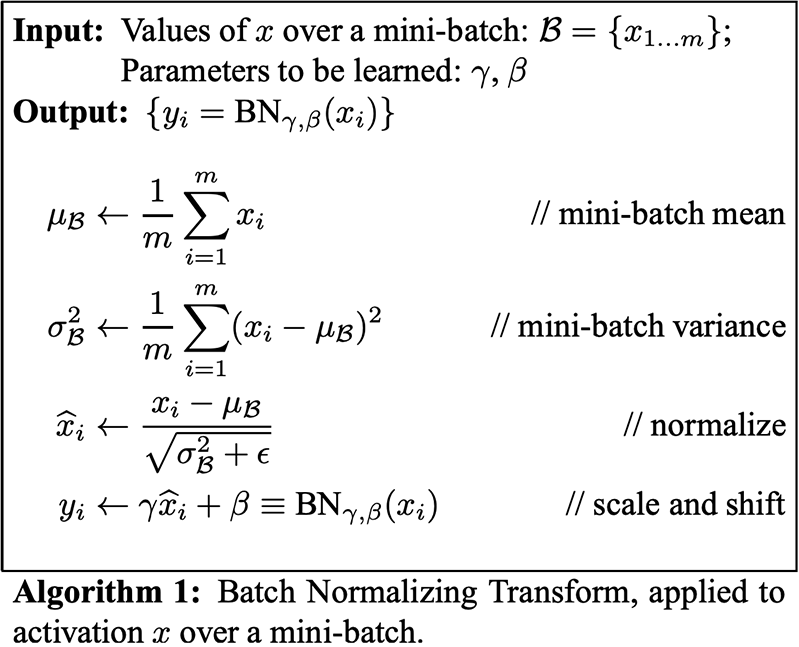
\includegraphics[width=0.95\textwidth]{figures/batch_normlization_page_76}
	\end{center}
	\caption{Batch Normalization}\label{fig:batch_normalization}
\end{figure}


\paragraph{Transposed Convolution}


Ignoring channels for now, let’s begin with the basic transposed convolution operation with stride of 1 and no padding.
Suppose that we are given a input tensor \( n_{h} \times n_{w} \) and a  kernel \( k_{h} \times  k_{w} \).
Sliding the kernel window with stride of 1 for \( n_{w} \) times in each row and \( n_{h} \) times in each column yields a total of \( n_{h}n_{w} \) intermediate results.
Each intermediate result is a \( \left(n_{h} + k_{h} -1\right) \times  \left(n_{w} + k_{w} - 1\right) \) tensor that are initialized as zeros.
To compute each intermediate tensor, each element in the input tensor is multiplied by the kernel so that the resulting tensor \( k_{h} \times k_{w} \) replaces a portion in each intermediate tensor.
Note that the position of the replaced portion in each intermediate tensor corresponds to the position of the element in the input tensor used for the computation.
In the end, all the intermediate results are summed over to produce the output~\cite[Chapter~14.10]{zhang2023dive}.


\begin{figure}
	\begin{center}
		\includesvg[width=0.95\textwidth]{figures/trans_conv}
	\end{center}
	\caption{Transposed Convolution~\cite[Chapter~14.10]{zhang2023dive}}\label{fig:trans_conv}
\end{figure}


Different from in the regular convolution where padding is applied to input, it is applied to output in the transposed convolution.
For example, when specifying the padding number on either side of the height and width as 1, the first and last rows and columns will be removed from the transposed convolution output.


\begin{figure}
	\begin{center}
		\includesvg[width=0.95\textwidth]{figures/trans_conv_stride2}
	\end{center}
	\caption{Transposed convolution with a kernel with stride of \( 2 \times 2 \). The shaded portions are a portion of an intermediate tensor as well as the input and kernel tensor elements used for the computation.~\cite{zhang2023dive}}\label{fig:trans_conv_stide}
\end{figure}


Consider implementing the convolution by multiplying matrices.
Given an input vector \( \mathbf{x} \) and a weight matrix \( \mathbf{W} \), the forward propagation function of the convolution can be implemented by multiplying its input with the weight matrix and outputting a vector \( y = \mathbf{W}\mathbf{x} \).
Since backpropagation follows the chain rule and \( \nabla_{x}\mathbf{y} = \mathbf{W}^{\top}\), the backpropagation function of the convolution can be implemented by multiplying its input with the transposed weight matrix \( \mathbf{W}^{\top}\) .
Therefore, the transposed convolutional layer can just exchange the forward propagation function and the backpropagation function of the convolutional layer: its forward propagation and backpropagation functions multiply their input vector with \( \mathbf{W}^{\top}  \) and \( \mathbf{W} \), respectively~\cite{zhang2023dive}.




\part{Algorithm and Data Structure}
\chapter{Algorithm}\label{chp:Algorithm}
\minitoc

\section{Graph}


\part{Programming}
\chapter{Leetcode}\label{chp:leetcode}
\minitoc

\section{Problems Sets}


\begin{itemize}
	\item \url{https://leetcode.com/list/rab78cw1/ https://www.techinterviewhandbook.org/grind75?weeks=8}
	\item dfs recursive = bfs iterative (use stack)
	\item two pointer
	\item check size (is\_empty, compare, larger, .etc.)
	\item hash map (fixed array)
\end{itemize}

\section{Tips}

\begin{itemize}
	\item postorder: LRN
	\item preorder: NLR
	\item inorder: LNR
	\item virtual head pointers
	\item two pointers (left and right, fast and slow)
	\item BST (value of left child is smaller, that of right child is larger)
	\item Backtracking (terminated option, available paths, current paths, if has
	\item duplicates(available paths or result))
	\item BFS (queue;while;for)
	\item sliding windows (tow pointers) for substring problems
	\item best-time-to-buy-and-sell-template.cpp
	\item (p + m - 1) / m equal to ceil(p / m)
	\item be careful about int overflow and underflow
	\item binary search problem: 1. left, right, f(x) increase/decrease, target
\end{itemize}

\section{Problems}

\subsection{ 1 Two Sum}

\begin{itemize}
	\item hash map
\end{itemize}

\subsection{20 valid parentheses}

\begin{itemize}
	\item  stack
\end{itemize}

\subsection{21 Merge Two Sorted List}

\begin{itemize}
	\item  recursive
\end{itemize}

\subsection{121 Best time to buy and sell stock}

\begin{itemize}
	\item record value
\end{itemize}

\subsection{226 Invert Binary Tree}

\begin{itemize}
	\item DFS recursive
	\item BFS iterative via stack
\end{itemize}

\subsection{242 Valid Anagram}

\begin{itemize}
	\item count freq then verify freq
\end{itemize}

\subsection{704 Binary Search}
\begin{itemize}
	\item two pointers
\end{itemize}

\subsection{733 Flood Fill}

\begin{itemize}
	\item graph matrix
	\item DFS via recursive or BFS via iterative
\end{itemize}

\subsection{235 lowest-common-ancestor-of-a-binary-search-tree}

\begin{itemize}
	\item Attributes of BST, the value of left subtree is less than root, that of left larger than root.
	\item Recursive
	\item iterative
\end{itemize}

\subsection{110 balanced-binary-tree}

\begin{itemize}
	\item recursive DFS
	\item use -1 means unbalanced
\end{itemize}

\subsection{141 linked-list-cycle}

\begin{itemize}
	\item two points fast and slow
	\item check if they meet again

\end{itemize}

\subsection{232 implement-queue-using-stacks}

\begin{itemize}
	\item Two stacks, input and output
	\item move when output is empty
	\item amortized cost for each operation is O(1).
\end{itemize}

\subsection{278 first-bad-version}

\begin{itemize}
	\item Binary Search
	\item use val directly instead of index
\end{itemize}

\subsection{383 ransom-note}

\begin{itemize}
	\item hash map (fixed array)
	\item check size first
\end{itemize}

\subsection{70 climbing-stairs}

\begin{itemize}
	\item Fibonacci like
	\item recursive (from top to down, memorization)
	\item iterative (from bottom to top, space O(1))
\end{itemize}

\subsection{409 longest-palindrome}

\begin{itemize}
	\item use even char freq
	\item cal odd char freq \(\left(\textrm{s.size()} - \textrm{odd} + \left(\textrm{odd} > 0\right)\right)\)
\end{itemize}

\subsection{206 reverse-linked-list}

\begin{itemize}
	\item recursive
	\item iterative (three pointes (prev, curr,next))
\end{itemize}

\subsection{169 majority-element}

\begin{itemize}
	\item moorse vote
\end{itemize}

\subsection{67 add-binary}

\begin{itemize}
	\item carry
	\item ASCII to int, vicewise
\end{itemize}

\subsection{543 diameter-of-binary-tree}

\begin{itemize}
	\item postorder traversal
\end{itemize}

\subsection{876 middle-of-the-linked-list}

\begin{itemize}
	\item fast and slow pointers
	\item get n and n/2 at same time
\end{itemize}

\subsection{104 maximum-depth-of-binary-tree}

\begin{itemize}
	\item DFS recursive
	\item postorder
\end{itemize}

\subsection{217 contains-duplicate}

\begin{itemize}
	\item Hash set
	\item unorder\_map to hash map
	\item map to BST
\end{itemize}

\subsection{53 maximum-subarray}

\begin{itemize}
	\item DP
	\item use subproblem to fix global problem
\end{itemize}

\subsection{57 insert-interval}

\begin{itemize}
	\item three situations
	\item not|overlap|not
\end{itemize}

\subsection{542 01-matrix}

\begin{itemize}
	\item DP first left top, then bottom, right
	\item BFS, first 0, then unseen
\end{itemize}

\subsection{973 k-closest-points-to-origin}

\begin{itemize}
	\item sort/n\_element/partial\_sort
	\item max-heap
	\item randomized quicksort
\end{itemize}

\subsection{3 longest-substring-without-repeating-characters}

\begin{itemize}
	\item slide window (two points)
\end{itemize}

\subsection{15 3sum}

\begin{itemize}
	\item sort
	\item two points
\end{itemize}

\subsection{102 binary-tree-level-order-traversal}

\begin{itemize}
	\item stack/queue BFS
	\item DFS recursive / keep level
\end{itemize}

\subsection{133 clone-graph}

\begin{itemize}
	\item DFS
	\item Amazing
\end{itemize}

\subsection{207 course-schedule}

\begin{itemize}
	\item \url{https://www.geeksforgeeks.org/kahns-algorithm-vs-dfs-approach-a-comparative-analysis/}
	\item BFS kahn's algorithm topological sort
	\item DFS better for larger V
	\item topological sort
\end{itemize}

\subsection{322 coin-change}

\begin{itemize}
	\item DP
\end{itemize}

\subsection{238 product-of-array-except-self}

\begin{itemize}
	\item prefix
	\item suffix
	\item space O(1)
\end{itemize}

\subsection{155 min-stack}

\begin{itemize}
	\item keep value and min at the same time
\end{itemize}

\subsection{98 validate-binary-search-tree}

\begin{itemize}
	\item Recursive
\end{itemize}

\subsection{200 number-of-islands}

\begin{itemize}
	\item find 1 and DFS clear 1
\end{itemize}

\subsection{33 search-in-rotated-sorted-array}

\begin{itemize}
	\item Binary Search
	\item check if mid and target are in same side
	\item if not same side assume one side is inf/-inf value let left/right advanced
\end{itemize}

\subsection{39 combination-sum}

\begin{itemize}
	\item Backtracking
\end{itemize}

\subsection{86.partition-list}

\begin{itemize}
	\item dummy pointers
	\item two pointers
\end{itemize}

\subsection{23.merge-k-sorted-lists}

\begin{itemize}
	\item heap/priority\_queue
	\item merge two lists iteratively
\end{itemize}

\subsection{142.linked-list-cycle-ii.cpp}

\begin{itemize}
	\item two pointers
\end{itemize}

\subsection{160.intersection-of-two-linked-lists.cpp}

\begin{itemize}
	\item contact two lists
	\item make sure two lists have same distance from the end
\end{itemize}

\subsection{26.remove-duplicates-from-sorted-array}

\begin{itemize}
	\item fast and slow pointers
\end{itemize}

\subsection{27.remove-element.cpp}

\begin{itemize}
	\item fast and slow pointers
\end{itemize}

\subsection{283.move-zeroes.cpp}

\begin{itemize}
	\item fast and slow pointers
	\item snowball
\end{itemize}

\subsection{5.longest-palindromic-substring}

\begin{itemize}
	\item dp
	\item two pointers (expand from center/narrow from both sides)
\end{itemize}

\subsection{669.trim-a-binary-search-tree.cpp}

\begin{itemize}
	\item BST (value of left child is smaller, that of right child is larger)
	\item postorder
\end{itemize}

\subsection{124.binary-tree-maximum-path-sum.cpp}

\begin{itemize}
	\item postorder
	\item discard nodes with negative value
\end{itemize}

\subsection{46.permutations.cpp}

\begin{itemize}
	\item Backtracking
\end{itemize}

\subsection{51.n-queens.cpp}

\begin{itemize}
	\item Backtracking(current path, options, terminated option)
\end{itemize}

\subsection{78.subsets.cpp}

\begin{itemize}
	\item backtracking
\end{itemize}

\subsection{77.combinations.cpp}

\begin{itemize}
	\item backtracking
\end{itemize}

\subsection{90.subsets-ii.cpp}

\begin{itemize}
	\item backtracking
\end{itemize}

\subsection{40.combination-sum-ii.cpp}

\begin{itemize}
	\item backtracking
\end{itemize}

\subsection{47.permutations-ii.cpp}

\begin{itemize}
	\item backtracking
\end{itemize}

\subsection{111.minimum-depth-of-binary-tree.cpp}

\begin{itemize}
	\item BFS
\end{itemize}

\subsection{752.open-the-lock.cpp}

\begin{itemize}
	\item BFS
\end{itemize}

\subsection{76.minimum-window-substring.cpp}

\begin{itemize}
	\item sliding windows
\end{itemize}

\subsection{438.find-all-anagrams-in-a-string.cpp}

\begin{itemize}
	\item sliding windows
\end{itemize}

\subsection{337.house-robber-iii.cpp}
\begin{itemize}

	\item 213.house-robber-ii.cpp
	\item 198.house-robber.cpp
	\item DP
	\item recursive with memorization
	\item DP table -> optimize table
\end{itemize}

\subsection{116. Populating Next Right Pointers in Each Node}

\begin{itemize}
	\item Three children tree traverse
	\item BFS \(O\left(N\right)\)  space \(O\left(1\right)\)
\end{itemize}

\chapter{C++}\label{chp:c++}
\minitoc


\section{Code Snippets}

\subsection{Random Number Generation}

\begin{minted}{cpp}
#include <algorithm>
#include <iostream>
#include <iterator>
#include <random>

int main() {
  std::random_device rd;
  std::mt19937 rng(rd());
  std::uniform_int_distribution<int> dist6(1, 6);
  std::generate_n(std::ostream_iterator<int>(std::cout, " "), 10,
                  [&dist6, &rng]() { return dist6(rng); });
  return 0;
}
\end{minted}


\subsection{Quick Sort}

\begin{minted}{cpp}
#include <vector>
using std::vector;

class Solution {
public:
    void sort(vector<int>& nums, int low, int high){
        if (low >= high)  return;

        int p = partition(nums, low, high);

        sort(nums, low, p - 1); // Changed p to p-1
        sort(nums, p + 1, high);
    }

    int partition(vector<int>& nums, int low, int high){
        int pivot  = low, l = pivot + 1, r = high;

        while(l <= r) {
            if (nums[l] < nums[pivot]) ++l;
            else if (nums[r] >= nums[pivot]) --r;
            else std::swap(nums[l], nums[r]);
        }
        std::swap(nums[pivot], nums[r]);
        return r;
    }

    void shuffle(vector<int>& nums){
        std::srand((unsigned) time(nullptr));
        int n = nums.size();

        for (int i = 0; i < n; ++i){
            int r = i + rand() % (n - i);
            std::swap(nums[i], nums[r]);
        }
    }

    vector<int> sortArray(vector<int>& nums) {
        shuffle(nums); // Shuffle the array before sorting
        sort(nums, 0, nums.size() - 1); // Changed nums.size() to nums.size() - 1
        return nums;
    }
};
\end{minted}

On average, the algorithm takes $O\left(n\log n\right)$ time. In the worst case, it takes $O\left(n^2\right)$ time.
We shuffle the array before sorting to avoid the worst case.


\chapter{Rust}\label{chp:Rust}
\minitoc


\part{Research}
\chapter{Paper Writing}\label{chp:paper_writing}
\minitoc


\section{Resources}

\begin{itemize}
	\item \url{https://github.com/MLNLP-World/Paper-Writing-Tips}
	\item \url{https://github.com/dspinellis/latex-advice}
	\item \url{https://www.tldraw.com}
	\item \url{https://github.com/guanyingc/latex_paper_writing_tips}
	\item \url{https://github.com/guanyingc/cv_rebuttal_template}
	\item \url{https://www.overleaf.com/gallery/tagged/tikz/page}
	\item \url{https://color.adobe.com/zh/explore}
	\item \url{https://github.com/acmi-lab/cmu-10717-the-art-of-the-paper/tree/main/resources}
\end{itemize}


\section{Writing Tips}


\begin{itemize}
	\item e.g. means \enquote{for example}.
	\item i.e. means \enquote{that is}.
	\item et al. means \enquote{and others of the same kind}.
	\item etc. means \enquote{and others}, do not specify people.
\end{itemize}

\paragraph{Avoid extreme meaning words}

\begin{table}[ht]
	\centering
	\begin{tabular}{@{}ll@{}}
		\toprule
		Original Term    & Alternative Terms                        \\
		\midrule
		obvious          & straightforward                          \\
		always           & usually, generally, often                \\
		never            & seldom, rare                             \\
		avoid, eliminate & reduce, mitigate, alleviate, relieve     \\
		a lot of         & much, many                               \\
		do (verb)        & perform, conduct, carry out              \\
		big              & large, significant                       \\
		like             & such as, for example                     \\
		think            & believe, consider, argue, claim, suggest \\
		talk             & discuss, describe, present, show         \\
		look at          & examine, investigate, explore, study     \\
		get              & obtain, acquire, receive, gain           \\
		keep             & maintain, retain, preserve               \\
		climb            & increase, rise, grow, improve, ascend    \\
		really           & very, extremely, highly                  \\
		\bottomrule
	\end{tabular}
	\caption{Alternative Terms for Common Words}
	\label{tab:alternative_terms}
\end{table}


\begin{enumerate}
	\item  Don’t spend too much time reading other people’s research, waiting for inspiration to strike you.
	      \begin{enumerate}
		      \item  Reading research should be a regular part of any economist’s routine.
		      \item But it is not a substitute for doing your own.
	      \end{enumerate}

	\item Don’t set the bar too high. You don’t need to win the Nobel.
	\item  But don’t set the bar too low!
	      \begin{enumerate}
		      \item Be wary of picking a topic that is of interest to a small number of people (e.g. you and your adviser).
		      \item In particular, think about topics that will interest those beyond this island
	      \end{enumerate}
	\item Your ideas and results won’t sell themselves.
	\item How you communicate your work is of crucial importance.
	\item There is no point in having an interesting piece of research that nobody understands or sees the point of.
	\item Many economists think of themselves as primarily experts in technical methods: Econometrics, economic theory, data expertise.
	\item This “white coat” mentality—that we are mainly scientists who then do a write-up of our results—is deeply wrong.
	\item Writing is an essential part of the research process, not a last-minute thing to be rushed.
\end{enumerate}

\paragraph{Latex Writing Tips}

\begin{itemize}
	\item use \verb|\usepackage{microtype}| to improve the appearance of the text.
	\item use \verb|\tablename~\ref{tab}| to reference table.
	\item use \verb|\figurename~\ref{fig}| to reference figure.
	\item \verb|Eq.~\eqref{eq1}|
	\item comments from different people can be distinguished by different colors. \verb|\newcommand{\yl}[1]{{\color{blue}{[(YL): #1]}}}|
\end{itemize}

\section{PhD Theses TIPs}


The PhD Thesis Tips from \url{https://www.karlwhelan.com/Teaching/PhD/phd-writing-talk.pdf}.

What makes a good thesis? Forget about objectivity—beauty is in the eye of the beholder.
A good thesis is one that readers think is good.
So, you need to explain well what you are doing to somebody else.
Your ideas and results won’t sell themselves.
How you communicate your work is of crucial importance.
There is no point in having an interesting piece of research that nobody understands or sees the point of.
The “white coat” mentality—that we are mainly scientists who then do a write-up of our results—is misguided.
Writing is an essential part of the research process, not a last-minute thing to be rushed.
This is particularly true of PhD theses which are read very carefully by externs, who are hoping that you have explained what you have done in a clear fashion.

\paragraph{Writing Skills: More Important Than You Think}
What makes a good thesis? Forget about objectivity—beauty is in the eye of the beholder.
A good thesis is one that readers think is good.
So, you need to explain well what you are doing to somebody else Your ideas and results won’t sell themselves. How you communicate your work is of crucial importance.
There is no point in having an interesting piece of research that nobody understands or sees the point of.
The  ``white coat" mentality—that we are mainly scientists who then do a write-up of our results—is misguided.
Writing is an essential part of the research process, not a last-minute thing to be rushed.
This is particularly true of PhD theses which are read very carefully by externs, who are hoping that you have explained what you have done in a clear fashion.

\paragraph{Start by Avoiding Very Bad Writing}
People can be quite sensitive about their writing.
If you are a native English speaker and you have a degree, you probably think you know how to write and communicate well.
Chances are, you might be wrong.
Most MA graduates and even many professional PhD-qualified economists write very poorly.
Good writing is hard to define. Bad writing is easy to spot.
A badly-written thesis will have:
\begin{enumerate}
	\item Mis-spelled words.
	\item Missing words.
	\item Sentences that don’t make sense or aren’t proper sentences.
	\item Poor use of punctuation – full stops, commas etc.
\end{enumerate}
This annoys the reader because it makes things harder to read (and understand) but also because it’s so easy to prevent.
It suggests you didn’t take the time to be careful.

\paragraph{What To Do About It?}
Read, re-read, edit, and re-edit.
And do this as you go along.
Read and edit after you’ve written a page or so.
This can correct most of the common errors of style, grammar, and spelling that occur in the writing process.
Most of you actually do know what a sentence is.
In addition to catching typos, a quick re-read and edit allows you to check that what you’ve written gets across what you’ve been trying to say.
Sometimes you can think you’ve made a point clearly but then you read what you’ve written and it’s not so good.
Read your stuff aloud or slowly to yourself.
Does it sound right? Are you writing proper sentences? Are you over-using jargon or certain particular phrases?
Use spell checks but don’t rely on them.
Grammar. There are rules about how to use commas, colons, semi-colons, full stops, about what defines a sentence. Try to learn them.

\section{Abstract}


\section{Introduction}

\begin{enumerate}
	\item Introductions are crucial because they set up the reader to understand what your topic is and what you are going to do in your paper.
	\item Quickly explain two things:
	      \begin{enumerate}
		      \item Why is the topic of your paper interesting?
		      \item What did YOU do? What is YOUR contribution? A new question? An existing question but new methodology? Existing question, existing methodology, new data (e.g. no previous Irish application)?
	      \end{enumerate}

	\item Be willing to give an outline of what your results are but don’t get into too many details.
	\item Because of its importance, spend a lot of time on the introduction.
	\item But don’t make it too long. Three pages is a limit. Two is better.
	\item I often start writing the introduction as soon I have some results and then keep adjusting it as the paper evolves.
	\item Conclusions, on the other hand, should be kept short and to the point. Don’t repeat lots of stuff from the intro.
\end{enumerate}

\section{Literature Reviews}

\begin{enumerate}
	\item You need to explain your contribution.
	\item So it needs to be put in context.
	\item This will require discussion of previous studies in this area.
	\item Remember, though, the purpose is to set up your contribution, and distinguish it from previous work.
	\item Don’t simply provide a long list of separate descriptions of weakly related studies. (X (2007) did this. Y(2009) did that ...)
	\item Grouping studies together by type may be a better way of explaining it than listing lots of separate individual studies.
	\item A well-focused literature review is usually a useful component of a PhD thesis. It shows externs and your supervisor that you have read the literature.
	\item However, it is not essential that articles submitted for publication have a literature review. You may be able to summarise the existing literature in your introduction or work it into your opening section that sets up what you are doing.
\end{enumerate}

\section{Method}



\section{Result}




\section{Conclusion}


\part{Book Reading}
\chapter{Dive into Deep Learning}\label{chp:dive-into-deep-learning}

\section{Linear Neural Networks}\label{sec:Linear Neural Networks}

\subsection{Exercise 3.1.6}

\paragraph{Exercise 1:}

Let’s solve this analytically.

To minimize the sum of squared differences, we take the derivative of the function with respect to (b), set it equal to zero, and solve for (b).
The function to minimize is:

\[
	f(b) = \sum_{i=1}^{n} \left(x_i - b\right)^2
\]

Taking the derivative with respect to (b) gives:

\[
	f'(b) = \sum_{i=1}^{n} -2\left(x_i - b\right)
\]

Setting this equal to zero and solving for (b) gives:

\[
	0 = \sum_{i=1}^{n} -2(x_i - b)
\]
Solving for (b) gives:
\[
	b = \frac{1}{n} \sum_{i=1}^{n} x_i
\]

So the value of (b) that minimizes the sum of squared differences is the mean of the \(x_i\).

This problem and its solution relate to the normal distribution because the sum of squared differences is the basis for the maximum likelihood estimation of the mean of a normal distribution.
In other words, the mean of a normal distribution is the value that maximizes the likelihood of the observed data, which is equivalent to minimizing the sum of squared differences from the mean.


If we change the loss function to the sum of absolute differences, the problem becomes finding the median of the \(x_i\).
This is because the median is the value that minimizes the sum of absolute differences.
Unlike the mean, the median is not sensitive to extreme values, so it is a more robust measure of central tendency when there are outliers in the data.

\paragraph{Exercise 2:}

An affine function is a function composed of a linear transformation and a translation.
In the context of machine learning, an affine function often takes the form \(f(\mathbf{x}) = \mathbf{x}^\top \mathbf{w} + b)\), where \(\mathbf{x}\) is an input vector, \(\mathbf{w}\) is a weight vector, and (b) is a bias term.

We can show that this affine function is equivalent to a linear function on the augmented vector \((\mathbf{x}, 1)\) by considering a new weight vector \(\mathbf{w}' = (\mathbf{w}, b)\) and an augmented input vector \(\mathbf{x}' = (\mathbf{x}, 1)\).
Then the affine function can be written as a linear function:

\[
	f(\mathbf{x}) = \mathbf{x}^\top \mathbf{w} + b = \mathbf{x}'^\top \mathbf{w}'
\]


Here’s the proof:

The original affine function is \(f(\mathbf{x}) = \mathbf{x}^\top \mathbf{w} + b\).

We define \(\mathbf{x}' = (\mathbf{x}, 1)) and (\mathbf{w}' = (\mathbf{w}, b)\).

The dot product \(\mathbf{x}'^\top \mathbf{w}') is (\mathbf{x}^\top \mathbf{w} + 1 \cdot b\), which is exactly the original affine function.

Therefore, the affine function \(\mathbf{x}^\top \mathbf{w} + b\) is equivalent to the linear function \(\mathbf{x}'^\top \mathbf{w}'\) on the augmented vector \((\mathbf{x}, 1)\).
This equivalence is often used in machine learning to simplify the notation and the implementation of algorithms.

\paragraph{Exercise 3:}

A quadratic function of the form \(f(\mathbf{x}) = b + \sum_i w_i x_i + \sum_{j \leq i} w_{ij} x_{i} x_{j}\) can be implemented in a deep network using a fully connected layer followed by an element-wise multiplication operation and another fully connected layer.
Here’s how you can do it:

Input Layer: The input to the network is the vector \(\mathbf{x}\).

First Fully Connected Layer: This layer applies a linear transformation to the input vector.
The weights of this layer represent the \(w_i\) terms in the quadratic function. The output of this layer is \(b + \sum_i w_i x_i\).

Element-wise Multiplication Layer: This layer computes the element-wise product of the input vector with itself, resulting in the vector \(\mathbf{x} \odot \mathbf{x}\), where \(\odot\) denotes element-wise multiplication.
This operation corresponds to the \(x_i x_j\) terms in the quadratic function.

Second Fully Connected Layer: This layer applies a linear transformation to the output of the element-wise multiplication layer.
The weights of this layer represent the \(w_{ij}\) terms in the quadratic function. The output of this layer is \(\sum_{j \leq i} w_{ij} x_{i} x_{j}\).

Summation Layer: This layer adds the outputs of the first fully connected layer and the second fully connected layer to produce the final output of the network, which is the value of the quadratic function.

Note that this network does not include any activation functions, because the quadratic function is a polynomial function, not a nonlinear function.
If you want to model a more complex relationship between the input and the output, you can add activation functions to the network.

\paragraph{Exercise 4:}

If the design matrix \(\mathbf{X}^\top \mathbf{X}\) does not have full rank, it means that there are linearly dependent columns in the matrix \(\mathbf{X}\). This can lead to several problems:

The matrix \(\mathbf{X}^\top \mathbf{X}\) is not invertible, which means that the normal equations used to solve the linear regression problem do not have a unique solution.
This makes it impossible to find a unique set of regression coefficients that minimize the sum of squared residuals.

The presence of linearly dependent columns in \(\mathbf{X}\) can lead to overfitting, as the model can “learn” to use these redundant features to perfectly fit the training data, but it will not generalize well to new data.

One common way to fix this issue is to add a small amount of noise to the entries of \(\mathbf{X}\).
This can help to make the columns of \(\mathbf{X}\) linearly independent, which ensures that \(\mathbf{X}^\top \mathbf{X}\) has full rank and is invertible.
Another common approach is to use regularization techniques, such as ridge regression or lasso regression, which add a penalty term to the loss function that discourages the model from assigning too much importance to any one feature.

If you add a small amount of coordinate-wise independent Gaussian noise to all entries of \(\mathbf{X}\), the expected value of the design matrix \(\mathbf{X}^\top \mathbf{X}\) remains the same.
This is because the expected value of a Gaussian random variable is its mean, and adding a constant to a random variable shifts its mean by that constant. So if the noise has mean zero, the expected value of \(\mathbf{X}^\top \mathbf{X}\) does not change.

Stochastic gradient descent (SGD) can still be used when \(\mathbf{X}^\top \mathbf{X}\) does not have full rank, but it may not converge to a unique solution.
This is because SGD does not rely on the invertibility of \(\mathbf{X}^\top \mathbf{X}\), but instead iteratively updates the regression coefficients based on a randomly selected subset of the data.
However, the presence of linearly dependent columns in \(\mathbf{X}\) can cause the loss surface to have multiple minima, which means that SGD may converge to different solutions depending on the initial values of the regression coefficients.


\paragraph{Exercise 5:}

The negative log-likelihood of the data under the model is given by:

The likelihood function for the data is \(P(\mathbf y \mid \mathbf X) = \prod_{i=1}^{n} \frac{1}{2} \exp(-|y_i - (\mathbf x_i^\top \mathbf w + b)|)\), where \(y_i\) is the (i)-th target value, \(\mathbf x_i\) is the (i)-th input vector, \(\mathbf w\) is the weight vector, and (b) is the bias term.

Taking the negative logarithm of this gives the negative log-likelihood:

\(-\log P(\mathbf y \mid \mathbf X) = \sum_{i=1}^{n} \left( \log 2 + |y_i - (\mathbf x_i^\top \mathbf w + b)| \right)\).

Unfortunately, there is no closed-form solution for this problem.
The absolute value in the log-likelihood function makes it non-differentiable at zero, which means that we cannot set its derivative equal to zero and solve for \(\mathbf w\) and \(b\).

A minibatch stochastic gradient descent algorithm to solve this problem would involve the following steps:
Initialize \(\mathbf w\) and \(b\) with random values.
For each minibatch of data:
Compute the gradient of the negative log-likelihood with respect to \(\mathbf w\) and \(b\).
The gradient will be different depending on whether \(y_i - (\mathbf x_i^\top \mathbf w + b)\) is positive or negative.
Update \(\mathbf w\) and \(b\) by taking a step in the direction of the negative gradient.
Repeat until the algorithm converges.
One issue that could arise with this algorithm is that the updates could become very large if \(y_i - (\mathbf x_i^\top \mathbf w + b)\) is close to zero, because the gradient of the absolute value function is not defined at zero. This could cause the algorithm to diverge.

One possible solution to this problem is to use a variant of gradient descent that includes a regularization term, such as gradient descent with momentum or RMSProp.
These algorithms modify the update rule to prevent the updates from becoming too large.
Another solution is to add a small constant to the absolute value inside the logarithm to ensure that it is always differentiable.


\paragraph{Exercise 6:}

The composition of two linear layers in a neural network essentially results in another linear layer. This is due to the property of linearity: the composition of two linear functions is another linear function.

Mathematically, if we have two linear layers \(L_1\) and \(L_2\) such that \(L_1(x) = Ax + b\) and \(L_2(x) = Cx + d\), then the composition \(L_2(L_1(x)) = L_2(Ax + b) = C(Ax + b) + d = (CA)x + (Cb + d)\), which is another linear function.

This means that a neural network with two linear layers has the same expressive power as a neural network with a single linear layer. It cannot model complex, non-linear relationships between the input and the output.

To overcome this limitation, we typically introduce non-linearities between the linear layers in the form of activation functions, such as the ReLU (Rectified Linear Unit), sigmoid, or tanh functions. These non-linear activation functions allow the neural network to model complex, non-linear relationships and greatly increase its expressive power.

\paragraph{Exercise 7:}

Regression for realistic price estimation of houses or stock prices can be challenging due to the complex nature of these markets. Prices can be influenced by a wide range of factors, many of which may not be easily quantifiable or available for use in a regression model.

The additive Gaussian noise assumption may not be appropriate for several reasons.
First, prices cannot be negative, but a Gaussian distribution is defined over the entire real line, meaning it allows for negative values.
Second, the Gaussian distribution is symmetric, but price changes in real markets are often not symmetric.
For example, prices may be more likely to increase slowly but decrease rapidly, leading to a skewed distribution of price changes.
Finally, the Gaussian distribution assumes that large changes are extremely unlikely, but in real markets, large price fluctuations can and do occur.

Regression to the logarithm of the price can be a better approach because it can help to address some of the issues with the Gaussian noise assumption.
Taking the logarithm of the prices can help to stabilize the variance of the price changes and make the distribution of price changes more symmetric.
It also ensures that the predicted prices are always positive, since the exponential of any real number is positive.

When dealing with penny stocks, or stocks with very low prices, there are several additional factors to consider.
One issue is that the prices of these stocks may not be able to change smoothly due to the minimum tick size, or the smallest increment by which the price can change.
This can lead to a discontinuous distribution of price changes, which is not well modeled by a Gaussian distribution.
Another issue is that penny stocks are often less liquid than higher-priced stocks, meaning there may not be enough buyers or sellers to trade at all possible prices.
This can lead to large price jumps, which are also not well modeled by a Gaussian distribution.

The Black-Scholes model for option pricing is a celebrated model in financial economics that makes specific assumptions about the distribution of stock prices.
It assumes that the logarithm of the stock price follows a geometric Brownian motion, which implies that the stock price itself follows a log-normal distribution.
This model has been very influential, but it has also been criticized for its assumptions, which may not hold in real markets.
For example, it assumes that the volatility of the stock price is constant, which is often not the case in reality.

\paragraph{Exercise 8:}

The Gaussian additive noise model may not be appropriate for estimating the number of apples sold in a grocery store for several reasons:
The Gaussian model allows for negative values, but the number of apples sold cannot be negative.
The Gaussian model is a continuous distribution, but the number of apples sold is a discrete quantity.
The Gaussian model assumes that large deviations from the mean are extremely unlikely, but in reality, there could be large fluctuations in the number of apples sold due to various factors (e.g., seasonal demand, promotions).

The Poisson distribution is a discrete probability distribution that expresses the probability of a given number of events (in this case, the number of apples sold) occurring in a fixed interval of time or space.
The parameter \(\lambda\) is the rate at which events occur.
The expected value of a Poisson-distributed random variable is indeed \(\lambda\). This can be shown as follows:

The expected value (E[k]) of a random variable (k) distributed according to a Poisson distribution is given by:

\[E[k] = \sum_{k=0}^{\infty} k \cdot p(k \mid \lambda) = \sum_{k=0}^{\infty} k \cdot \frac{\lambda^k e^{-\lambda}}{k!}\]

By the properties of the Poisson distribution, this sum equals \(\lambda\).

The loss function associated with the Poisson distribution is typically the negative log-likelihood. Given observed counts \(y_1, y_2, \ldots, y_n\) and predicted rates \(\lambda_1, \lambda_2, \ldots, \lambda_n\), the negative log-likelihood is:

\[L(\lambda, y) = \sum_{i=1}^{n} \left(\lambda_i - y_i \log \lambda_i\right)\]

If we want to estimate \(\log \lambda\) instead of \(\lambda\), we can modify the loss function accordingly.
One possible choice is to use the squared difference between the logarithm of the predicted rate and the logarithm of the observed count:

\[L\left(\log \lambda, y\right) = \sum_{i=1}^{n} \left(\log \lambda_i - \log y_i\right)^2\]

This loss function penalizes relative errors in the prediction of the rate, rather than absolute errors. It can be more appropriate when the counts vary over a wide range, as it gives equal weight to proportional errors in the prediction of small and large counts.

\subsection{Exercise 3.3.5}

\paragraph{1. What will happen if the number of examples cannot be divided by the batch size. How would you change this behavior by specifying a different argument by using the framework’s API?}

PyTorch: In PyTorch's \emph{DataLoader}, there's an argument called \emph{drop\_last}.
If set to True, it will drop the last incomplete batch.
By default, it's set to \emph{False}.

\begin{minted}{python}
train_loader = torch.utils.data.DataLoader(dataset, batch_size=batch_size,
    shuffle=True, drop_last=True)
\end{minted}

\paragraph{2. Suppose that we want to generate a huge dataset, where both the size of the parameter vector w and the number of examples num\_examples are large.}

1. What happens if we cannot hold all data in memory?

2. How would you shuffle the data if it is held on disk? Your task is to design an efficient algorithm that does not require too many random reads or writes.
Hint: pseudorandom permutation generators 75 allow you to design a reshuffle without the need to store the permutation table explicitly (Naor and Reingold, 1999).

1. What happens if we cannot hold all data in memory?

If we cannot hold all the data in memory:

\textbf{Performance Impact}: Reading data directly from disk is much slower than reading from memory. If the training algorithm frequently accesses the disk, it can significantly slow down the training process.

\textbf{Out-of-Core Processing}: You'll need to use "out-of-core" or "external memory" algorithms, which are designed to process data that is too large to fit into a computer's main memory.
These algorithms break the data into smaller chunks that can fit into memory, process each chunk, and then combine the results.

\textbf{Streaming:} Data can be streamed from the disk in mini-batches.
Only one mini-batch is loaded into memory at a time, and after processing it, the next mini-batch is loaded.
This is common in deep learning when dealing with large datasets.

\textbf{Distributed Computing}: Another approach is to distribute the dataset across multiple machines in a cluster.
Each machine processes a subset of the data. Frameworks like TensorFlow and PyTorch have support for distributed training.

2. How would you shuffle the data if it is held on disk?

Shuffling large datasets on disk without too many random reads or writes can be challenging. Here's a method using pseudorandom permutation generators:

1. Pseudorandom Permutation: Use a pseudorandom permutation generator to generate a sequence of indices that represents the shuffled order of your data.
The beauty of pseudorandom permutation generators is that they can generate the nth element of the sequence without generating the first n-1 elements, allowing for efficient random access.

2. Sequential Reads and Writes:
- Read the data from the disk sequentially in large chunks (to benefit from sequential read speeds).
- For each item in the chunk, use the pseudorandom permutation generator to determine its new location in the shuffled dataset.
- Write the shuffled data back to the disk sequentially in large chunks.

3. In-Place Shuffling: If you have some memory available (but not enough to hold the entire dataset), you can load chunks of data into memory, shuffle them using the pseudorandom permutation, and then write them back to disk.
This reduces the number of disk writes.

4. External Sorting: Another approach is to use techniques from external sorting.
Divide the data into chunks that fit into memory, shuffle each chunk in memory, and then merge the chunks together in a shuffled manner.

5. Temporary Storage: If possible, use a fast intermediate storage (like an SSD) to temporarily store data chunks during the shuffling process.
This can speed up both reads and writes.

Remember, the key is to minimize random disk accesses, as they are much slower than sequential accesses.
Leveraging pseudorandom permutations allows for an efficient reshuffling without the need to store large permutation tables explicitly.


\paragraph{3. Implement a data generator that produces new data on the fly, every time the iterator is called.}

\begin{minted}{python}
import torch
from torch.utils.data import Dataset, DataLoader

class RandomDataset(Dataset):
    def __init__(self, num_samples, tensor_size):
        """
        Args:
            num_samples (int): Number of samples in the dataset.
            tensor_size (tuple): Size of the tensor to be generated.
        """
        self.num_samples = num_samples
        self.tensor_size = tensor_size

    def __len__(self):
        return self.num_samples

    def __getitem__(self, idx):
        # Generate a random tensor on the fly
        sample = torch.randn(self.tensor_size)
        return sample

# Parameters
num_samples = 1000
tensor_size = (3, 32, 32)  # Example: 3-channel, 32x32 image

# Create dataset and dataloader
random_dataset = RandomDataset(num_samples, tensor_size)
dataloader = DataLoader(random_dataset, batch_size=32, shuffle=True)

# Iterate over the dataloader
for batch in dataloader:
    print(batch.shape)  # Should print torch.Size([32, 3, 32, 32])
                        # for all batches except possibly the last one
\end{minted}

\paragraph{4. How would you design a random data generator that generates the same data each time it is called?}

\begin{minted}{python}
torch.manual_seed(idx)
\end{minted}


\subsection{Exercise 3.5.6}

\paragraph{1. How would you need to change the learning rate if you replace the aggregate loss over the minibatch with an average over the loss on the minibatch?}

When you replace the aggregate loss over the minibatch with an average over the loss on the minibatch, you're essentially scaling the loss by a factor of \( \frac{1}{\text{batch size}} \).
If you're using gradient descent or a variant thereof, the update rule is:

\[ \theta_{\text{new}} = \theta_{\text{old}} - \eta \nabla L \]

Where:
- \( \theta \) represents the parameters of the model.
- \( \eta \) is the learning rate.
- \( \nabla L \) is the gradient of the loss function \( L \) with respect to the parameters.

If you change the loss from an aggregate to an average, the gradient \( \nabla L \) will also be scaled by \( \frac{1}{\text{batch size}} \). To compensate for this scaling and to ensure that the magnitude of the parameter updates remains the same, you would need to multiply the learning rate \( \eta \) by the batch size.

In other words, if your original learning rate was \( \eta_{\text{original}} \) when using aggregate loss, and you switch to using average loss, your new learning rate should be:

\[ \eta_{\text{new}} = \eta_{\textrm{original}} \times \textrm{batch size} \]

However, in practice, many deep learning frameworks, including TensorFlow and PyTorch, compute the average loss over a minibatch by default.
So, if you're already using one of these frameworks, you likely don't need to adjust the learning rate when switching between aggregate and average loss, unless you were explicitly scaling the loss by the batch size yourself.

\paragraph{4. What is the effect on the solution if you change the learning rate and the number of epochs? Does it keep on improving?}

The learning rate and the number of epochs are two critical hyperparameters in training neural networks and other machine learning models. Their values can significantly impact the convergence and performance of the model. Let's discuss the effects of changing each:

1. Learning Rate (\( \eta \)):
- Too High: If the learning rate is set too high, the model might overshoot the minima in the loss landscape, leading to divergence. The loss might oscillate or even explode.
- Too Low: If the learning rate is too low, the model will converge very slowly. It might get stuck in local minima or plateaus in the loss landscape.
- Adaptive: Many modern optimizers (like Adam, RMSprop) adjust the learning rate dynamically based on recent gradients, which can help in finding a good balance.

2. Number of Epochs:
- Too Few: If the number of epochs is too low, the model might underfit the data, as it hasn't seen the data enough times to learn the underlying patterns.
- Too Many: If the number of epochs is too high, the model might overfit the data, especially if there isn't an early stopping mechanism or regularization in place. Overfitting means the model performs well on the training data but poorly on unseen data.

Does it keep on improving?

- Not necessarily. As training progresses:
- The loss typically decreases and the model's performance on the training set improves.
- However, after a certain point, the model might start to overfit, and its performance on a validation set might start to degrade.
- The optimal number of epochs is often where the performance on the validation set is maximized.

- The learning rate plays a crucial role in this:
- A good learning rate can help the model converge to a good solution faster.
- Learning rate schedules or decay can be beneficial. Starting with a larger learning rate (to progress quickly) and reducing it over time (to fine-tune) can be effective.

In summary, there's a balance to strike.
It's essential to monitor both training and validation metrics during training to determine the best values for the learning rate and the number of epochs.
Experimentation and hyperparameter tuning, possibly with techniques like cross-validation or Bayesian optimization, can help find the optimal values for a given problem and dataset.


\subsection{Exercise 4.1.5}

\paragraph{1. We can explore the connection between exponential families and softmax in some more depth}

1. Compute the second derivative of the cross-entropy loss \(l(y, \hat{y})\) for softmax.
2. Compute the variance of the distribution given by softmax(o) and show that it matches the second derivative computed above.

1. Second Derivative of Cross-Entropy Loss for Softmax, The cross-entropy loss for softmax is given by:

\[ l(y, \hat{y}) = - \sum_{i} y_i \log(\hat{y}_i) \]

Where \( \hat{y}_i \) is the softmax output:

\[ \hat{y}_i = \frac{\exp(o_i)}{\sum_j \exp(o_j)} \]

Let's compute the second derivative with respect to the logits \( o \).

First, the derivative of \( \hat{y}_i \) with respect to \( o_k \) is:

\[ \frac{\partial \hat{y}_i}{\partial o_k} = \hat{y}_i (\delta_{ik} - \hat{y}_k) \]

Where \( \delta_{ik} \) is the Kronecker delta (it's when \( i = k \) and 0 otherwise).
Using the above, the second derivative is:

\[ \frac{\partial^2 l}{\partial o_i \partial o_k} = -\sum_j y_j \frac{\partial^2 \log(\hat{y}_j)}{\partial o_i \partial o_k} \]

\[ = -\sum_j y_j \frac{\partial}{\partial o_i} \left( \frac{\hat{y}_j (\delta_{jk} - \hat{y}_k)}{\hat{y}_j} \right) \]

\[ = -\sum_j y_j \left(\delta_{jk} - \hat{y}_k\right) \frac{\partial \hat{y}_j}{\partial o_i} \]

\[ = -\sum_j y_j \left(\delta_{jk} - \hat{y}_k\right) \hat{y}_j \left(\delta_{ji} - \hat{y}_i\right) \]

2. Variance of the Distribution Given by Softmax

The variance \( \textrm{Var}[X] \) of a discrete random variable \( X \) with possible outcomes \( x_1, x_2, \ldots \) and probabilities \( p_1, p_2, \ldots \) is:

\[ \textrm{Var}[X] = \sum_i p_i \left(x_i - \mathbb{E}[X]\right)^2 \]

For the softmax distribution, \( X \) can take on values corresponding to the logits \( o \) with probabilities \( \hat{y} \). Thus, the variance becomes:

\[ \textrm{Var}[X] = \sum_i \hat{y}_i \left(o_i - \mathbb{E}[X]\right)^2 \]

Where \( \mathbb{E}[X] = \sum_i \hat{y}_i o_i \).

Now, the second derivative of the cross-entropy loss with respect to the logits, as derived above, gives us a measure of the curvature of the loss.
When we compare this with the variance of the softmax distribution, we can see that they are related. The variance captures the spread of the logits, and the second derivative captures the sensitivity of the loss to changes in the logits. In the context of exponential families, this relationship between variance and the second derivative of the log-likelihood is a known property.

To show that they match, one would equate the expressions derived in the two sections above and simplify.
The detailed algebra can be quite involved, but the key insight is understanding the relationship between the curvature of the loss (second derivative) and the spread of the logits (variance).


\paragraph{5. Softmax gets its name from the following mapping: \(RealSoftMax(a, b) = log(exp(a) + exp(b))\)}

1. Prove that \( \textrm{RealSoftMax}(a, b) > \max(a, b) \):

Given:
\[ \textrm{RealSoftMax}(a, b) = \log(\exp(a) + \exp(b)) \]

Now, since \( \exp(a) \) and \( \exp(b) \) are both positive, we have:
\[ \exp(a) + \exp(b) > \exp(a) \]
\[ \exp(a) + \exp(b) > \exp(b) \]

Taking the logarithm of both sides (logarithm is a monotonically increasing function):
\[ \log(\exp(a) + \exp(b)) > \log(\exp(a)) = a \]
\[ \log(\exp(a) + \exp(b)) > \log(\exp(b)) = b \]

Thus, \( \text{RealSoftMax}(a, b) > \max(a, b) \).

2. How small can you make the difference between both functions?

Without loss of generality, let's set \( b = 0 \) and \( a \geq b \). Then:
\[ \textrm{RealSoftMax}(a, 0) = \log(\exp(a) + 1) \]

The difference between the two functions is:
\[ \textrm{RealSoftMax}(a, 0) - a = \log(\exp(a) + 1) - a \]

As \( a \) becomes large, the difference approaches 0, but it's always positive because of the "+1" inside the logarithm.

3. Prove that this holds for \( \lambda^{-1} \textrm{RealSoftMax}\left(\lambda a, \lambda b\right) \), provided that \( \lambda > 0 \):

Given:
\[ \lambda^{-1} \textrm{RealSoftMax}\left(\lambda a, \lambda b\right) = \lambda^{-1} \log(\exp(\lambda a) + \exp(\lambda b)) \]

Using the property of logarithms:
\[ = \log(\exp(\lambda a) + \exp(\lambda b))^{\lambda^{-1}} \]

Since \( \exp(\lambda a) \) and \( \exp(\lambda b) \) are both positive and \( \lambda > 0 \), the proof from part  applies here as well, and we can conclude that \( \lambda^{-1} \textrm{RealSoftMax}(\lambda a, \lambda b) > \max(a, b) \).

4. Show that for \( \lambda \to \infty \) we have \( \lambda^{-1} \textrm{RealSoftMax}(\lambda a, \lambda b) \to \max(a, b) \):

As \( \lambda \) becomes very large, the term \( \exp(\lambda a) \) will dominate \( \exp(\lambda b) \) if \( a > b \). Thus:
\[ \lambda^{-1} \log(\exp(\lambda a) + \exp(\lambda b)) \approx \lambda^{-1} \log(\exp(\lambda a)) = a \]

Similarly, if \( b > a \), the result will be \( b \).
Therefore, as \( \lambda \to \infty \), \( \lambda^{-1} \textrm{RealSoftMax}(\lambda a, \lambda b) \to \max(a, b) \).

5. Construct an analogous softmin function:

The softmin function can be constructed using the negative of the inputs to the softmax function:
\[ \textrm{RealSoftMin}(a, b) = -\textrm{RealSoftMax}(-a, -b) \]
\[ = \log(\exp(-a) + \exp(-b)) \]

6. Extend this to more than two numbers:

For \( n \) numbers \( a_1, a_2, \ldots, a_n \):
\[ \textrm{RealSoftMax}(a_1, a_2, \ldots, a_n) = \log(\exp(a_1) + \exp(a_2) + \ldots + \exp(a_n)) \]

Similarly, the softmin for \( n \) numbers is:
\[ \textrm{RealSoftMin}(a_1, a_2, \ldots, a_n) = \log(\exp(-a_1) + \exp(-a_2) + \ldots + \exp(-a_n)) \]

\subsection{Exercise 4.5.5}

\paragraph{Deep learning uses many different number formats, including FP64 double precision (used extremely rarely), FP32 single precision, BFLOAT16 (good for compressed representations), FP16 (very unstable), TF32 (a new format from NVIDIA), and INT8. Compute the smallest and largest argument of the exponential function for which the result does not lead to numerical underflow or overflow}

\begin{table}[h!]
	\centering
	\begin{tabular}{lrrrrrrr}
		\toprule
		format         & format\_min & format\_max & exp\_min   & exp\_max & test\_min & exp(max-1) & exp(max+1) \\
		\midrule
		torch.float64  & -1.80e+308  & 1.80e+308   & -1.80e+308 & 7.10e+02 & 0.00e+00  & 6.61e+307  & inf        \\
		torch.float32  & -3.40e+38   & 3.40e+38    & -3.40e+38  & 8.87e+01 & 0.00e+00  & 1.25e+38   & inf        \\
		torch.bfloat16 & -3.39e+38   & 3.39e+38    & -3.39e+38  & 8.85e+01 & 0.00e+00  & 1.00e+38   & inf        \\
		torch.float16  & -6.55e+04   & 6.55e+04    & -6.55e+04  & 1.11e+01 & 0.00e+00  & 2.41e+04   & inf        \\
		torch.int8     & -1.28e+02   & 1.27e+02    & -1.28e+02  & 4.84e+00 & 0.00e+00  & 4.67e+01   & 8.90e+01   \\
		\bottomrule
	\end{tabular}
\end{table}

1. FP64 (Double Precision):
- Smallest positive normalized number \(2^{-1022}\)
- Largest finite representable number \( (2-2^{-52}) \times 2^{1023} \)
- For the exponential function, the range of \(x\) for which \(e^x\) does not overflow would be approximately \([-1022 \log(2), 1023 \log(2)]\).

2. FP32 (Single Precision):
- Smallest positive normalized number: \(2^{-126}\)
- Largest finite representable number: \( (2-2^{-23}) \times 2^{127} \)
- For the exponential function, the range of \(x\) for which \(e^x\) does not overflow would be approximately \([-126 \log(2), 127 \log(2)]\).

3. BFLOAT16:
- This format has the same exponent bits as FP32 but fewer precision bits.
- The range for the exponential function would be similar to FP32.

4. FP16:
- Smallest positive normalized number: \(2^{-14}\)
- Largest finite representable number: \( (2-2^{-10}) \times 2^{15} \)
- For the exponential function, the range of \(x\) for which \(e^x\) does not overflow would be approximately \([-14 \log(2), 15 \log(2)]\).

5. TF32:
- This is a new format introduced by NVIDIA, and it has 10 bits for the exponent and 19 bits for the fraction.
- The range would be somewhere between FP32 and FP16.

6. INT8:
- This is an integer format, so it doesn't directly apply to the exponential function in the same way as the floating-point formats. However, if used in quantized neural networks, the range would be \([-128, 127]\).

For the exact ranges, especially for the newer formats like TF32, one would need to refer to the official documentation or specifications provided by the manufacturers.

To avoid overflow or underflow when computing the exponential function, it's common to clip or bound the input values to the function within the safe range for the given number format.

\subsection{Exercise 7.1.6}

\paragraph{1. Assume that the size of the convolution kernel is \(\Delta = 0 \). Show that in this case the convolution kernel implements an MLP independently for each set of channels. This leads to the Network in Network architectures}

When the size of the convolution kernel is \( \Delta = 0 \), it means that the kernel effectively has a size of \( 1 \times 1 \).
A \( 1 \times 1 \) convolution kernel operates on each pixel individually, without considering its neighbors.

Let's break down the implications of this:

1. Independent Operation on Each Pixel: A \( 1 \times 1 \) convolution operates on each pixel independently.
For an input with \( C_{in} \) channels, each pixel is represented by a \( C_{in} \)-dimensional vector.
The \( 1 \times 1 \) convolution transforms this \( C_{in} \)-dimensional vector into a \( C_{out} \)-dimensional vector, where \( C_{out} \) is the number of output channels.

2. MLP for Each Set of Channels: The transformation from \( C_{in} \) to \( C_{out} \) for each pixel can be viewed as a fully connected layer (or MLP) applied independently to each spatial location.
This is because the weights of the \( 1 \times 1 \) convolution kernel can be seen as the weights of a fully connected layer that connects each input channel to each output channel.

3. Network in Network (NiN): The idea of using \( 1 \times 1 \) convolutions to implement an MLP for each set of channels led to the Network in Network (NiN) architecture.
In NiN, multiple \( 1 \times 1 \) convolutional layers are stacked, allowing for deep per-pixel transformations. This introduces additional non-linearity for each pixel without changing the spatial dimensions.

In summary, a \( 1 \times 1 \) convolution kernel effectively applies an MLP to each pixel independently, transforming the channels at each spatial location.
This concept is central to the Network in Network (NiN) architecture, which uses \( 1 \times 1 \) convolutions to introduce additional non-linearities in the network without altering the spatial dimensions.

\paragraph{5. What happens with convolutions when an object is at the boundary of an image?}

When an object is at the boundary of an image, and we apply convolutions, several issues and considerations arise:

1. Loss of Information: The primary issue is that for pixels on the boundary, there aren't enough neighboring pixels to apply the convolution kernel fully.
This means that these boundary pixels might not be processed adequately, leading to potential loss of information about objects at the image boundary.

2. Padding: To address the boundary issue, one common approach is to add padding around the image. Padding involves adding extra pixels around the boundary of the image.
There are different types of padding:
- Zero Padding: Adding pixels with a value of zero.
- Reflect Padding: The boundary pixels are reflected. For instance, if the last row of an image is \([a, b, c]\), it becomes \([a, b, c, c, b, a]\) after reflect padding.
- Replicate Padding: The boundary pixels are replicated. Using the previous example, it becomes \([a, b, c, c, c, c]\).

Padding ensures that every pixel, including those on the boundary, has a full neighborhood of pixels to apply the convolution kernel.

3. Valid vs. Same Convolutions:
- Valid Convolution: No padding is used. The resulting feature map after convolution is smaller than the input image because the kernel can only be applied to positions where it fits entirely within the image boundaries.
- Same Convolution: Padding is added such that the output feature map has the same spatial dimensions as the input image.

4. Edge Effects: Even with padding, objects at the boundary might be affected differently than objects in the center of the image.
This is because the artificial values introduced by padding might not represent the actual image content. This can lead to edge artifacts in the output feature map.

5. Dilated Convolutions: In dilated convolutions, where the kernel elements are spaced out by introducing gaps, the boundary effects can be even more pronounced, especially if the dilation rate is high.

6. Pooling Layers: The boundary effects can also impact pooling layers (like max-pooling or average-pooling).
If the pooling window doesn't fit entirely within the image or feature map boundaries, padding might be needed, or the pooling window might be truncated.

\paragraph{6. Prove that the convolution is symmetric, \(f * g = g * f\)}

To prove that convolution is symmetric, we'll start with the definition of the convolution operation for two functions \( f(t) \) and \( g(t) \):

\[ \left(f * g\right)\left(t\right) = \int_{-\infty}^{\infty} f\left(\tau\right) g\left(t - \tau\right) \, d\tau \]

Now, let's express the convolution of \( g \) and \( f \):

\[ \left(g * f\right)\left(t\right) = \int_{-\infty}^{\infty} g\left(\tau\right) f\left(t - \tau\right) \, d\tau \]

To show that these two expressions are equivalent, we'll make a substitution:

Let \( \lambda = t - \tau \)
This implies \( d\lambda = -d\tau \)

When \( \tau = -\infty \), \( \lambda = t + \infty = \infty \)
When \( \tau = \infty \), \( \lambda = t - \infty = -\infty \)

Substituting these values into the convolution of \( g \) and \( f \), we get:

\[ (g * f)(t) = \int_{\infty}^{-\infty} g(t - \lambda) f(\lambda) (-d\lambda) \]

Now, reversing the limits of integration:

\[ (g * f)(t) = \int_{-\infty}^{\infty} g(t - \lambda) f(\lambda) \, d\lambda \]

Comparing this with the expression for \( (f * g)(t) \), we see that the two expressions are equivalent:

\[ (f * g)(t) = (g * f)(t) \]

Thus, we've proven that the convolution operation is symmetric:

\[ f * g = g * f \]


\paragraph{Exercise 7.2.8}

\paragraph{4. How do you represent a cross-correlation operation as a matrix multiplication by changing the input and kernel tensors?}

Cross-correlation can be represented as a matrix multiplication by converting the input and kernel tensors into appropriate matrix and vector forms, respectively.
This process is often referred to as ``toeplitzization'' or ``im2col'' (image to column) transformation. Here's how you can achieve this:

1. Flatten the Kernel:
- First, you reshape the kernel into a column vector.
- If the kernel is of size \( k \times k \), the resulting vector will be of size \( k^2 \times 1 \).

2. Toeplitz Matrix for Input:
- For each position in the output, extract a \( k \times k \) patch from the input, and flatten it into a row vector.
- Stack these row vectors on top of each other to form a matrix. This matrix has a special structure called a Toeplitz matrix.
- If the input is of size \( n \times n \) and the kernel is \( k \times k \), then the resulting matrix will be of size \( \left(n-k+1\right)^2   \times k^2 \).

3. Matrix Multiplication:
- Multiply the Toeplitz matrix (from step 2) with the flattened kernel (from step 1). The result will be a column vector representing the flattened output of the cross-correlation operation.
- Reshape this column vector back into a 2D matrix to get the final output.

Mathematically, if \( M \) is the Toeplitz matrix derived from the input and \( K \) is the column vector derived from the kernel, then the output \( O \) is given by:

\[ O = M \times K \]

This representation is particularly useful for certain computational platforms and algorithms that can efficiently handle matrix multiplications.
In deep learning frameworks, this transformation is often used under the hood to speed up convolution operations, especially when using GPUs.

Note: This explanation assumes 2D inputs and kernels for simplicity, but the concept can be extended to higher dimensions.

\begin{minted}{python}
def im2col(inputs, kernel_size):
    # Extract patches from the input tensor
    k, _ = kernel_size
    unfold = torch.nn.Unfold(kernel_size=k, stride=1, padding=0)
    cols = unfold(inputs)
    return cols.transpose(1, 2)
\end{minted}

% section Linear Neural Networks (end)


\begin{appendices}
	\chapter{Formulas}

\section{Gaussian distribution}\label{sec:gaussian_distribution}

\begin{definition}[Gaussian distribution]\label{def:gaussian_distribution}
	\myindex{Gaussian distribution}
\end{definition}

\begin{theorem}[Central limit theorem]\label{thm:central_limit_theorem}
\end{theorem}


\end{appendices}

\backmatter

%%%%%%%%%%%%%%% Reference %%%%%%%%%%%%%%%

\printbibliography[heading=bibintoc]
\printindex

\end{document}
